\documentclass[5p, times]{elsarticle}

%%%%%%%%%%%%%%   Preample  %%%%%%%%%%%%%%%%%%

%% The amssymb package provides various useful mathematical symbols
\usepackage{amssymb}
%% The amsthm package provides extended theorem environments
\usepackage{amsthm}
\usepackage{mathtools}

%% for celcius symbol
\usepackage{textcomp}

%% for units
\usepackage{siunitx}

%% The lineno packages adds line numbers. Start line numbering with
%% \begin{linenumbers},  end it with \end{linenumbers}. Or switch it on
%% for the whole article with \linenumbers.
\usepackage{lineno}
\modulolinenumbers[5]

\usepackage{hyperref}

%% package for type Greek letters without entering into math-mode
\usepackage{textgreek}

%% package for large picture in two-colume
\usepackage{dblfloatfix}
\usepackage{fixltx2e}
\usepackage{float}

\usepackage{comment}

%% only jpg pdf eps are allowed, tiff format are not allowed in latex
%% eps in principle can't be compiled by pdflatex, pdf not compiled by latex, but Kile can do some intermedate conversion to allow this happen.
\DeclareGraphicsExtensions{.pdf, .eps, .jpg}
%%opening
\journal{NIMA}

\begin{document}

%%%%%%%%%%%%%% Front Matter %%%%%%%%%%%%%%%%%%
\begin{frontmatter}

\title{Design and verification of a low power large dynamic readout unit for the PSD detector of DAMPE project}

\author[imp,lzu,ucas]{Yong Zhou}

\author[imp]{Yuhong Yu\corref{corresponding_author}}
\cortext[corresponding_author]{Corresponding author}
\ead{yuyuhong@impcas.ac.cn}

\author[imp]{Zhiyu Sun}
\author[imp]{Yongjie Zhang}
\author[imp]{Fang Fang}
\author[imp]{Junling Chen}

\author[lzu]{Bitao Hu}

\address[imp]{Institute of Modern Physics, Chinese Academy of Sciences,  509 Nanchang Road,  Lanzhou,  730000,  P.R.China}
\address[lzu]{School of Nuclear Science and Technology,  Lanzhou University,  222 South Tianshui Road,  Lanzhou,  730000,  P.R.China}
\address[ucas]{Graduate University of the Chinese Academy of Sciences,  19A Yuquan Road,  Beijing,  100049,  P.R.China}

%%
\begin{abstract}

\begin{comment}
A Plastic Scintillator Detector (PSD), consisting of individual 82 organic plastic scintillator strips with 1 cm thick,
located at the top of DAMPE (DArk Matter Particle Explore), has been developed. It mainly serves as anti-coincidence
detector, also as a charge detector to measure cosmic ray nuclei up to charge $Z=20$. A large dynamic range from \SI{0.1}{MIPs} to \SI{1400}{MIPs} has been deduced after consideration various contributions. 
Integrating of a PMT with double dynodes readout and an ASIC chip VA160, a large dynamic readout system has been presented. 
A cosmic ray muons and an accelerator beam test have been used to verify this design, respectively. 
The results show that the readout system could satisfy the required dynamic range. 
\end{comment}

A large dynamic range readout unit is developed for the Plastic Scintillator Detector(PSD) of DArk Matter Paricle Explorer(DAMPE).
By extracting the signal form dynode5 and dynode8 of the photomultiplier tube, the unit can cover the wide signal amplitude range of PSD(from electron to Z=20).
The design has been verified using cosmic ray muon and relativistic Ar beam at CERN.
A dynamic range from \SI{0.1}{MIPs} to \SI{1400}{MIPs} has been achieved.

\end{abstract}

%%
\begin{keyword}
plastic scintillator
\sep VA160
\sep large dynamic range
\sep double dynodes readout

%% PACS codes here,  in the form: \PACS code \sep codes

\end{keyword}

\end{frontmatter}

\linenumbers
%%%%%%%%%%%%%%%%  Introduction  %%%%%%%%%%%%%%%%%%%%%%%
\section{Introduction}
\label{sec:introduction}

DArk Matter Paricle Explorer(DAMPE) is a satellite-borne particle detector aiming for in-direct dark matter search, high-energy gamma astronomy and primary cosmic ray study~\cite{Chang_Jin_dampe}.
It is designed to cover a wide energy range, from \SI{5}{GeV} to \SI{10}{TeV} for electrons and photons and from \SI{10}{GeV} to \SI{1}{PeV} for heavy ions, with unprecedented resolution(\SI{1.5}{\percent} at \SI{100}{\giga\electronvolt}).
% By extending the measurement to the \si{TeV} region, DAMPE will complement current experimental results~\cite{guzik_advanced_1999,picozza2010instrument,aguilar2013first} and shed more light on the new phenomena in this region. 
The Plastic Scintillator Detector(PSD), which sits at the top of the satellite, is a key sub-detector of DAMPE.
It consists of two layers of plastic scintillator bars which are orthogonal to each other, and covers an effective detection area of $\SI{820}{mm}\times\SI{820}{mm}$.
The bars are made of EJ-200~\cite{scintillator} with the dimension of $\SI{884}{mm} \times \SI{28}{\milli\meter} \times \SI{10}{mm}$, and coupled to a Hamamatsu R4443 PMT~\cite{r4443} at both ends using \SI{3}{mm}-thick silicon rubber(EJ-560~\cite{scintillator}).

\begin{comment}
To fulfil the requirements and optimize performance, the readout unit of PSD needs a careful design, which is guided by the following rules:
\begin{itemize}
 \item Large dynamic range.To cover the signal amplitude from minimum ionizing electrons to relativistic calcium ions.
 \item Large signla-to-noise ratio(SNR).For efficient charged particle detection.
 \item Low power consumption. The whole PSD is limitted to 19W, 12W for the front end electronics and 7W for the detection units(high voltage distribution and PMT base circuit).
\end{itemize}
\end{comment}
By measuring the deposited energy, PSD serves as an anti-coincidence detector for e/$\gamma$ discrimination as well as a charge detector for heavy ions up to Z=20.
These functions impose harsh demands for the readout system of PSD, which, together with the PMT, needs to cover a wide range of signal amplitudes from singly charged minimum ionizing particles to relativistic calcium ions, while in the same time keeping sufficient resolution and large signal-to-noise ratio(SNR) for effective particle identification.   
As a space experiment, the power consumption of PSD is restricted to be $\leq$19W as a whole, 12W for the front end electronics(FEE) and 7W for the high voltage distribution and PMT base circuit.
This adds an extra constraint in the design of the readout unit.

In this paper, a low power and large dynamic range readout unit for PSD is reported.
Verification tests for the design have been carried out using cosmic ray and relativistic heavy ion beam, and the results are satisfactory.
The detailed description of the design is presented in Sec.\ref{sec:requirement} and Sec.\ref{sec:design}, and the test results are discussed in Sec.\ref{sec:result}.

%%%%%%%%%%%%%%%% Main Text Body %%%%%%%%%%%%%%%%%%%%%%%
\section{Dynamic range requirement}
\label{sec:requirement}

\begin{figure*}
\centering
 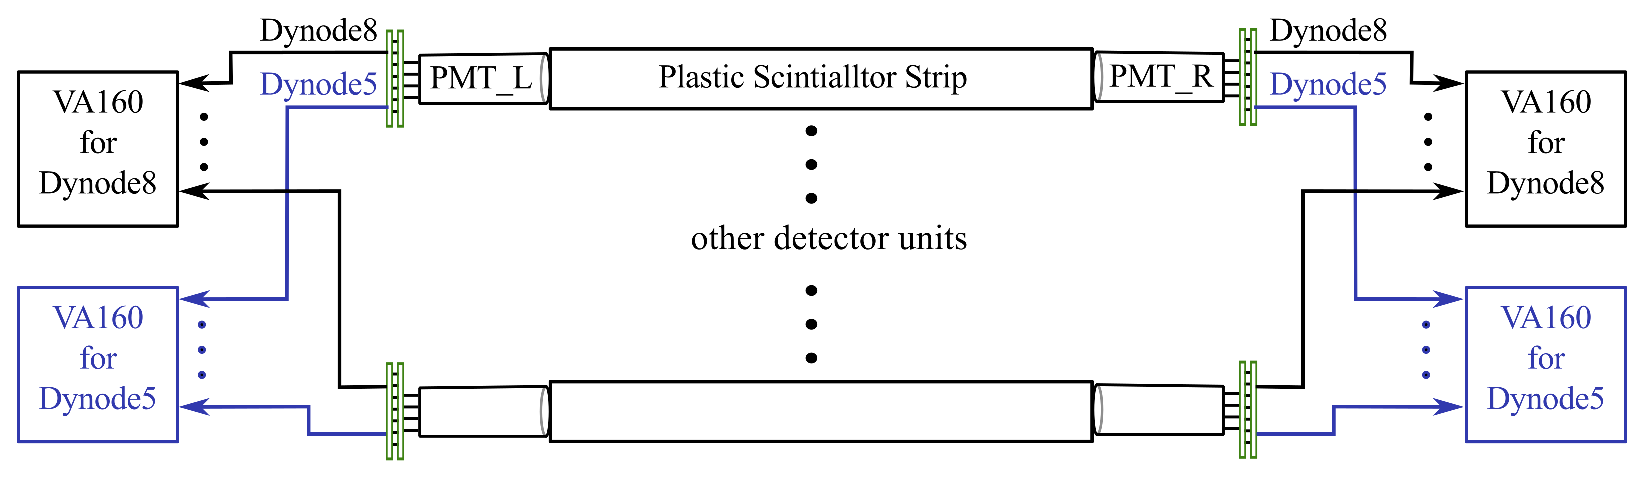
\includegraphics[width=140mm]{readout_scheme}
\caption{Readout scheme of PSD.}
\label{fig:readout_scheme}
\end{figure*} 

\begin{figure*}
\centering
 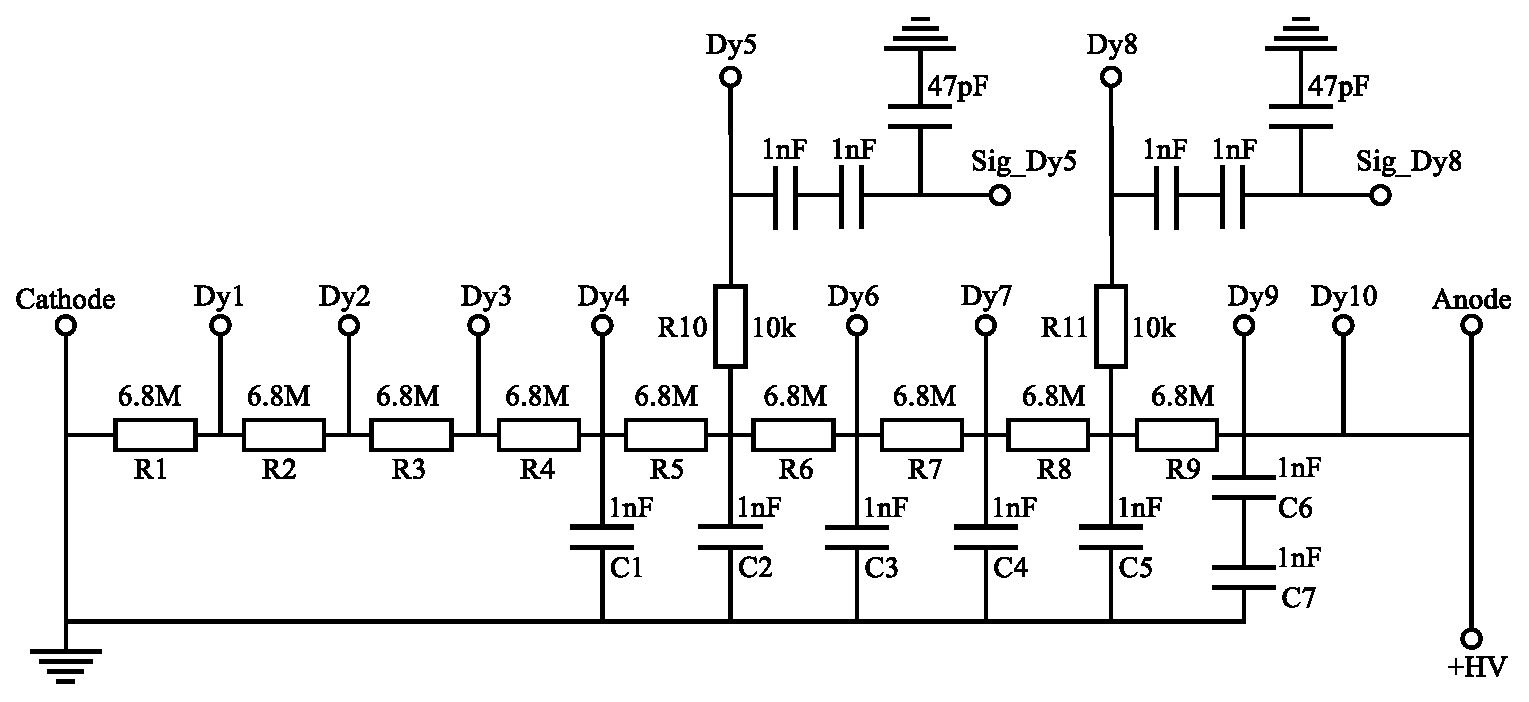
\includegraphics[width=140mm]{divider}
\caption{Circuit diagram of the voltage divider.}
\label{fig:divider}
\end{figure*} 

\begin{figure*}[t]
 \centering
 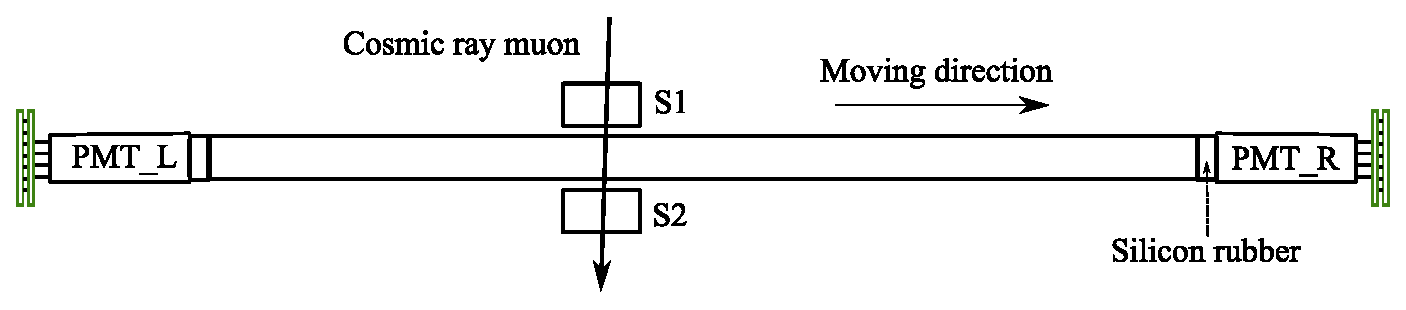
\includegraphics[width=140mm]{cosmic_test}
\caption{The experimental setup for the cosmic ray test.}
\label{fig:cosmic_test}
\end{figure*} 

\subsection{Light yield in response to relativistic heavy ions}
% According to the Bethe-Bloch equation~\cite{olive_review_2014}, the energy deposited in PSD bars is approximately proportional to $Z^2$ for particles heavier than electron.
The light yield of organic scintillators is a nonlinear function of the desposited energy $\Delta E$ due to the quenching effect.
It can be described precisely by the Birks law~\cite{birks_theory_2013} in the low energy range, while for heavy ions in the relativistic region, the scintillation mechanism gets much more complicated and the Birks law fails to apply.
Several modified models~\cite{chou_nature_1952,tarle_cosmic_1979,menchaca-rocha_response_1999,matsufuji_response_1999} have been proposed to extend the Birks law to the high energy region, nevertheless large discrepancy exists between them when extrapolating to the high-Z nuclides.

Due to the theoretical difficulties metioned above, our estimation of the light yield is based on the direct beam test result of AMS-02 TOF prototype~\cite{marrocchesi2011beam}, which also uses EJ-200 as the detection material and has the same thickness.
According to ~\cite{marrocchesi2011beam}, the light output of calcium is about 270 times larger than that of proton.
As all singly charged minimum ionization particles have approximately the same response in the plastic scintillator, this result indicates a maximum of 270 times difference in the light yield for all the particle species covered by PSD.

\subsection{Miscellaneous contributions to the dynamic range}

Actual dynamic range needed by PSD is expanded by several other contributions. 
To make things clear, we define the mean light yield produced by a singly charged minimum ionizing particle penetrating through vertically in the middle of the bar as one MIP, and use it as the unit for the dynamic range calculation.

The first contribution comes from DAMPE's broad field of view, which implies a maximum incidence angle of \SI{60}{\degree} for particles through PSD.
This doubles the travel length and thus the energy deposit in PSD, and expands the maximum light yield to \SI{540}{MIPs}.  
Secondly, the statistical nature of the ionizing process should be taken into account.
Assuming a full coverage of the energy fluctuation is 5$\sigma$ and $\sigma$=\SI{10}{\percent}, the dynamic range of light output expands to \SI{675}{MIPs} in the upper limit and \SI{0.75}{MIPs} in the lower limit. 
Finally, the long length of the scintillator bar makes the light attenuation non-negligible.
The bars are surface-polished and wrapped by the Tyvek paper to improve reflection efficiency, and preliminary tests show that the light reduction ratio between the middle position and the two ends can be well controlled above 0.5.
Thus, the light collected by the end PMTs will vary between \SI{0.375}{MIPs} and \SI{1350}{MIPs}.

To leave some redundancy for the adjustment, the final dynamic range required by the readout unit of PSD is determined to be \SI{0.1}{MIPs}$\sim$\SI{1400}{MIPs}.

\begin{comment}
\subsection{yuyuhong}
Many contributions would enlarge the required dynamic range. 
The energy deposition in the organic plastic scintillator and its scintillation efficiency is one of the most important contribution to the required dynamic range. 
When minimum ionizing particles (MIPs) passing through 1 cm thick scintillator strip, they release a certain amount of energy. 
This value is about 2 MeV~\cite{olive_review_2014}, defined as 1 MIPs. 
For a charge particle much heavier than electron the specific ionization energy loss is well parameterized by the famous Bethe-Bloch formula. 
The mean rate of energy loss increases with the charged number Z of the relativistic incident particle. 
However, the dependence of light output from energy deposition is usually nonlinear in organic plastic scintillator. 
A relationship between the response of the scintillator to a charged particle and the specific energy loss is well modeled by Briks-Chou law~\cite{birks1951scintillations,birks1964theory}. 

In order to know the quantitative information on the light output response of organic plastic scintillator to energetic heavy ions at relativistic energies, many experiments investigate this nonlinear effect~\cite{dwyer1985plastic,bindi2005performance,marrocchesi2011beam}. 
The maximum energy deposition in 1 cm thick scintillator strip at the PSD is about 270 MIPs from the charge of cosmic rays nuclei up to Z=20 when they travelling through the detector medium vertically. 
Moreover, a field view of DAMPE will determine the maximum length of incident charged particle, and this energy deposition is about 540 MIPs as the max incident inclination angle is approximately \SI{60}{\degree}.

Another contribution to the dynamic range of the energy deposition is the light attenuation in a long scintillator strip. 
In the case where a specific geometry and a wrapping material are given to the scintilltor strips at the PSD, the light attenuation is definite. 
After selection of the scintillator strip, a reduction ratio in the intensity of the scintillation light is hoped to smaller than 50\% as the incident particle hit the middle position perpendicularly.
Since two charge measurements are carried on with the PMTs placed in both sides of a given strip and these two PMTs are reserved for each other, a mean rate of energy deposition range from 0.5 MIPs to 1080 MIPs at least is required for cosmic ray nuclei from Z=1 up to Z=20.

The fluctuation of energy loss by ionization of a charged particle in a thin scintillator is also taken into account.
Assumption the energy resolution of the fluctuation($\sigma$) is \SI{10}{\percent}, a maximum measurable energy deposition per scintillator strip up to 1350 MIPs is required as a 5$\sigma $ width is accepted, while a minimum value down to 0.25 MIPs is required at least. 
Therefore, a readout system for each PSD unit covering a dynamic range from 0.1 MIPs to 1400 MIPs could meet all requirements.
\end{comment}

\section{Design of the readout unit}
\label{sec:design}

\subsection{Readout scheme}
% A variety of designs can be referenced to cover the large dynamic range of the detector outputs~\cite{katayose2008development,kampert1994high,genolini_low_2003}.
We have adopted the readout scheme based on multi-dynodes readout of R4443 singal.
Small singal is extracted by high-gain dynode and large signal is extracted by low-gain dynode.
To eliminate the cross-talk effect, singals from high gain dynodes and low gain dynodes will be processed by separate VA160 as shown in Fig.\ref{fig:readout_scheme}.
The scheme is simple and robust, minimal components are used.
As two VA160 channels are used, reserve the resolution.

VA160 is a highly integrated, low power consumption ASIC chip for charge measurement.
low noise, high sensitivity
It incorporates charge-sensitive amplifier, shaper
FEE board based VA160 has been developed by the Institute of Modern 

\subsection{Selection of the dynode stages}
% \subsection{Photon number of one MIP}


\subsection{Base circuit design and implementation}

Based on the previous discussion, a fully resistive voltage divider is designed to extract current pulses from dynode5 and dynode8, as shown in Fig.\ref{fig:divider}.
The decoupling capacitors $C_1\sim C_7$ are used to improve the linearity by compensating the charge required in the formation of large singals.
The ramping resistors $R_10$ and $R_11$ and bypass capacitors $C_10$ and $C_13$ are here to better form the output waveform.
Two coupling capacitors of the dynode readout circuit are serial chained together

\begin{comment}
It's difficult to read out a signal in such a wide range by using only one front-end electronics (FEE) circuit. 
There are several ways to achieve a high dynamic readout were reported~\cite{katayose2008development,kampert1994high,genolini_low_2003}. 
To measure the energy deposition in the range with 4 orders of magnitude at each plastic scintillator strip of PSD, a readout system that uses a PMT with double dynode outputs coupled to FEE with an ASIC chip has been developed and performed. 
A low power consumption ASIC chip known as VA160, which can be seen as a modified version of the VA32-HDR14.2, developed by IDEAS (Norway)~\cite{va160}, is used as the FEE for the PSD. 
This VA160 chip is optimized for positive input signals for the PMT dynodes output, and the analog to digital conversion is performed by a 14-bit ADC. 
The saturation level is about \SI{12}{\pico\coulomb}, and the RMS noise of this chip is about \SI{0.8}{\femto\coulomb}.

Among the PSD, those of the lower dynamic range \SI{0.1}{MIP} will be need to measure. 
An input noise of the PSD whole system about \SI{6}{\femto\coulomb} is expected for the detection of the incident particles. 
To distinguish signal from noise clearly, a $5\sigma$ separation of the detector pedestal is required, so we can deduce that 1 MIPs energy deposition should be better to set to \SI{300}{\femto\coulomb}. 
Thus a dynamic range from 0.1 MIPs to 40 MIPs can be achieved for one electronic channel.
This dynamic range could not cover the total required dynamic range, so a PMT with double dynodes readout is indispensible. 
Fig.~\ref{fig:readout_scheme} shows the combination of dual-gain photo devices and VA160 chip per each scintillator channel.
It’s shown that the signals from the same PMT are sent to different VA160 chip separately to reduce the crosstalk between the two dynodes.

As MIPs penetrating a long strip, the efficiency of light transmission is limited by total reflection angle, and that not more than \SI{22.5}{\percent} fraction of scintillation light would reach the two ends of the strip. 
Taking into account that the scintillator EJ-200 generates one photon for every 100 eV of deposited energy, we can calculate the number of photon electrons (PEs) collected by one end of PMT as MIPs penetrating 1 cm thick strip in the middle point from Eq.~\ref{eq:pecalculation}.
\begin{align}
 N_{PEs} &= \frac{1}{2} \times \frac{\SI[per-mode=symbol]{2}{\mega\electronvolt\per\centi\meter}}{\SI{100}{\electronvolt}} \times 0.225
           \times \varepsilon_{1} \times \varepsilon_{2} \times \varepsilon_{3} \times \varepsilon_{4} \times \SI{1}{\centi\meter} \nonumber \\
         &\approx \SI{45}{PEs/mip}
\label{eq:pecalculation}
\end{align} 
where $\varepsilon_1$ is the reduction ratio related to the intensity of the scintillation light between the hit position and the end of the strip, and this value is controlled to smaller than \SI{50}{\percent}.
The value of$\varepsilon_2$, corresponding to the quantum efficiency of the readout PMT, is about 0.15. 
The parameter $\varepsilon_3$ is the transmission ratio of a \SI{3}{\milli\meter} thick silicon rubber optical interface, and this value is approximately 0.9. 
The last parameter $\varepsilon_4$ is determined by the geometry efficiency, which is the ratio of the effective photocathode area of the readout device and the cross section of the scintillator strip, and the calculated value is approximately 0.3.

The chosen PMT R4443MOD2, composed of 10 stage dynodes, has a gain factor of $1.0\times 10^6$ at the supply high voltage of \SI{1000}{\volt}, which is obviously too high for the VA160 chip. 
Using the standard voltage divider and supply voltage from Hamamatsu, a simple calculation to obtain the multiplication factor of the two adjacent dynodes is 4. 
To match the dynamic range of VA160, the signal from the middle dynodes is extracted to reduce the gain factor of the PMT. 
The 8th dynode (Dy8), with a gain of $6\times 10^4$ from a rough calculation at given standard voltage, is the optimal selection to test the MIPs signals. 
The positive charge outputs from Dy8 is \SI{450}{\femto\coulomb}, which is a little larger than our expectation \SI{300}{\femto\coulomb}, and the difference can be eliminated easily by fine adjustment of the supply high voltage of the PMTs. 
To cover the required upper dynamic range, an earlier stage 5th dynode (Dy5) is used to the larger signals measurements, as the relative gain factor across three dynodes is 64 at standard supply voltage from a simple calculation. 
Since the operating voltage is smaller than the standard voltage, the relative gain of Dy8/Dy5 is expected to $50\pm15$ times. 
Assumption the relative gain between the two dynodes is 35 times, then the Dy5 will cover an energy range from 3.5 MIPs to 1400 MIPs. 
Therefore, the total readout system could achieve the demanded wide range of 4 orders, and also provide a cross calibration between the two dynodes. 
Figure 2 shows the circuit diagram of the PMT divider. 
It’s shown that the voltage distribution across the dynodes is the same. 
To improve the output linearity of the input pulse, decoupling capacitors are connected to the last few stages using a parallel mode. 
To protect the high voltage power, two capacitors in series are used in the output of dynodes.
\end{comment}


\section{Tests result}
\label{sec:result}

\subsection{Test with LED}

\subsection{Test with cosmic ray}
\label{sec:cosmicray}

Cosmic ray muons are the most numerous energetic charged at sea level with a mean energy of about 4 GeV, and are typically MIPs. 
As muons penetrating orthogonally in 1 cm scintillator, the amount of energy around 1 MIPs leaves on average per unit length. 
So a cosmic ray muons test was used to study the MIPs response at the laboratory. 
The layout of the test setup for a scintillator strip with cosmic ray muons is shown in Fig.~\ref{fig:cosmic_test}. 
Two small trigger, with the dimension of \ 1.0×1.0×1.0 cm\textsuperscript{3}, also made with scintillator are fixed on a movable support to investigate the performance of the readout system, and point-by-point measurement has been carried out. 

Fig.~\ref{fig:mip} shows a typical MIPs energy spectrum read out from Dy8. 
The amplitude spectrum has an asymmetric form with a longer right-hand tail which is characteristic for thin absorbers. 
The most probable amplitude of the distribution characterizing mean energy losses for MIPs is obtained by fitting a Landau function to the spectrum as shown in Fig.~\ref{fig:mip}. 
The most probable value of MIPs signals is 396.5 ADC counts. 
It’s approximately \SI{320}{\femto\coulomb} when the ADC count is converted into charge. 
The amplitude distribution of the pedestal for each signal channel is also shown in Fig.~\ref{fig:mip}.
From the Figure, we can find that the input noise of the whole PSD system is approximate 3 fC, which is merely half of the expected value. 
As a result of 0.1 MIPs signals, the most probable value of the signal-to-noise of the PSD system is greater than 10, and this value is exceeding the expected requirement for a 5$\sigma $ separation from the whole PSD detector pedestal.

\begin{figure}
 \centering
 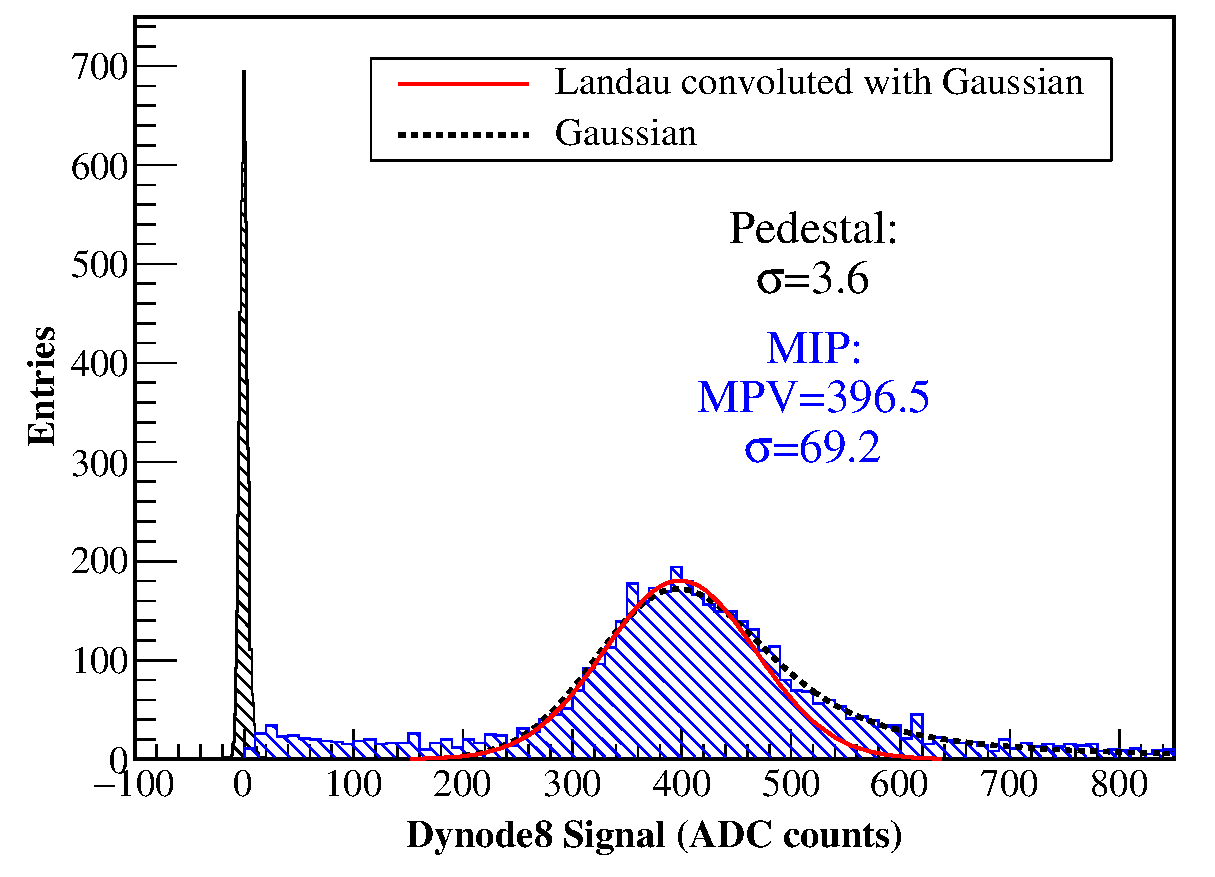
\includegraphics[width=90mm]{mip}
\caption{The pulse height distribution of cosmic muons from a low gain channel Dy8.}
\label{fig:mip}
\end{figure} 

The light attenuation of the scintillator strip could not be negligible for the required dynamic range. 
Fig.~\ref{fig:attenuation} shows the charge amplitude at various locations along the scintillator strip, and it’s found that the amplitude is well fitted by an exponent fit. 
In the figure, the charge amplitude at different hit locations is scaled to the middle hit position. 
It’s shown that the amplitude of charge pulse is not independent on the hit position. 
From the fitting data, the ratio between the nearest and the farthest hit position from the same readout PMT is not greater than 4, so it is not beyond the former desired value.

\begin{figure}
 \centering
 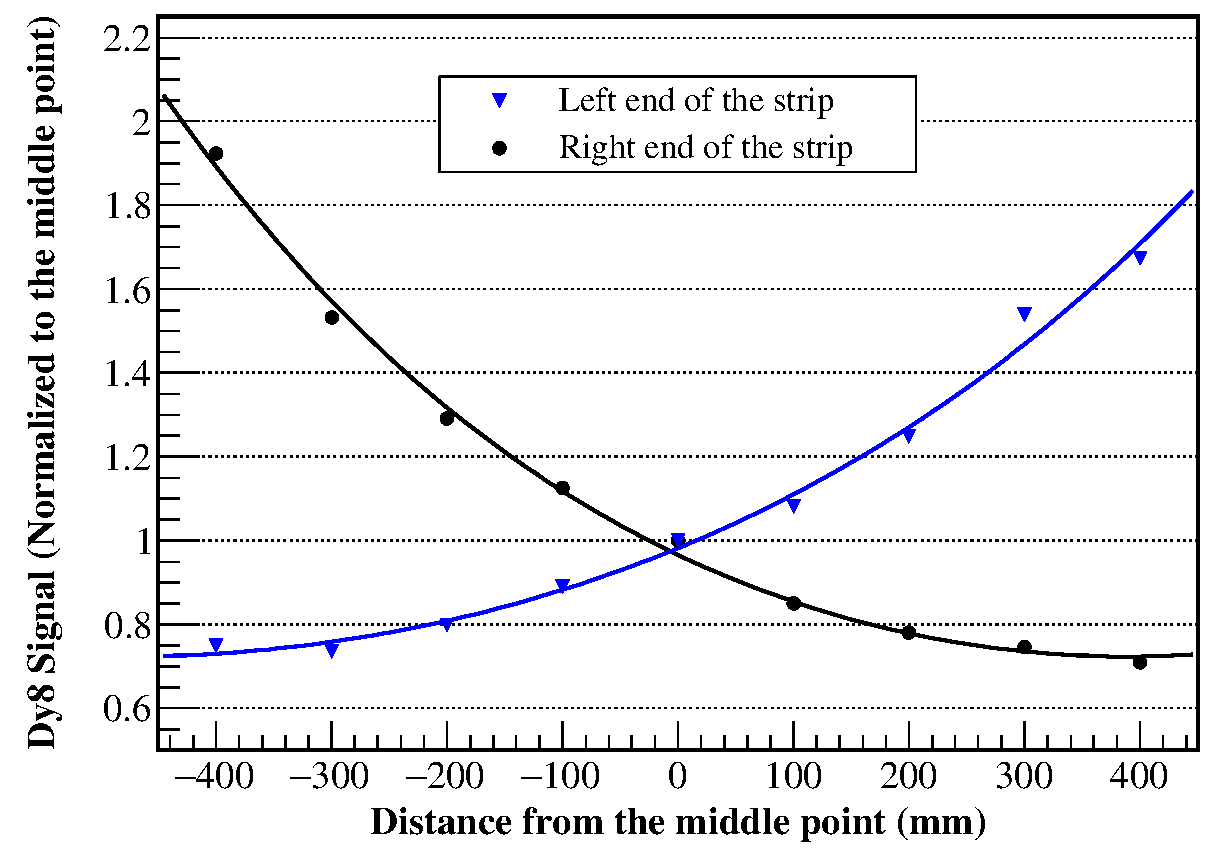
\includegraphics[width=90mm]{attenuation}
\caption{The charge pulse amplitude at different hit positions along the tested scintillator strip.}
\label{fig:attenuation}
\end{figure} 

The charge ratio of a low gain channel Dy8 and a high gain channel Dy5 is shown in Fig.~\ref{fig:dy58}. 
From figure, the charge collection of the Dy8 reach the maximum dynamic range of the VA160, and the saturation level is found to be about \SI{12}{\pico\coulomb}. 
From a linearity fit, the relative gain for Dy8/Dy5 of 44.6 could be derived, so the upper dynamic range of about 1670 MIPs can be obtained from a calculation using Eq.~\ref{eq:range}.
\begin{equation}
 Range_{upper} = k_{e}(Dy8/Dy5)
 \label{eq:range}
\end{equation} 
where $k_e$ is the VA160 charge dynamic range, and the adopted upper range of VA160 is \SI{12}{\pico\coulomb}.
Apparently, the required upper dynamic range1400 MIPs could be covered by our design.

\begin{figure}
 \centering
 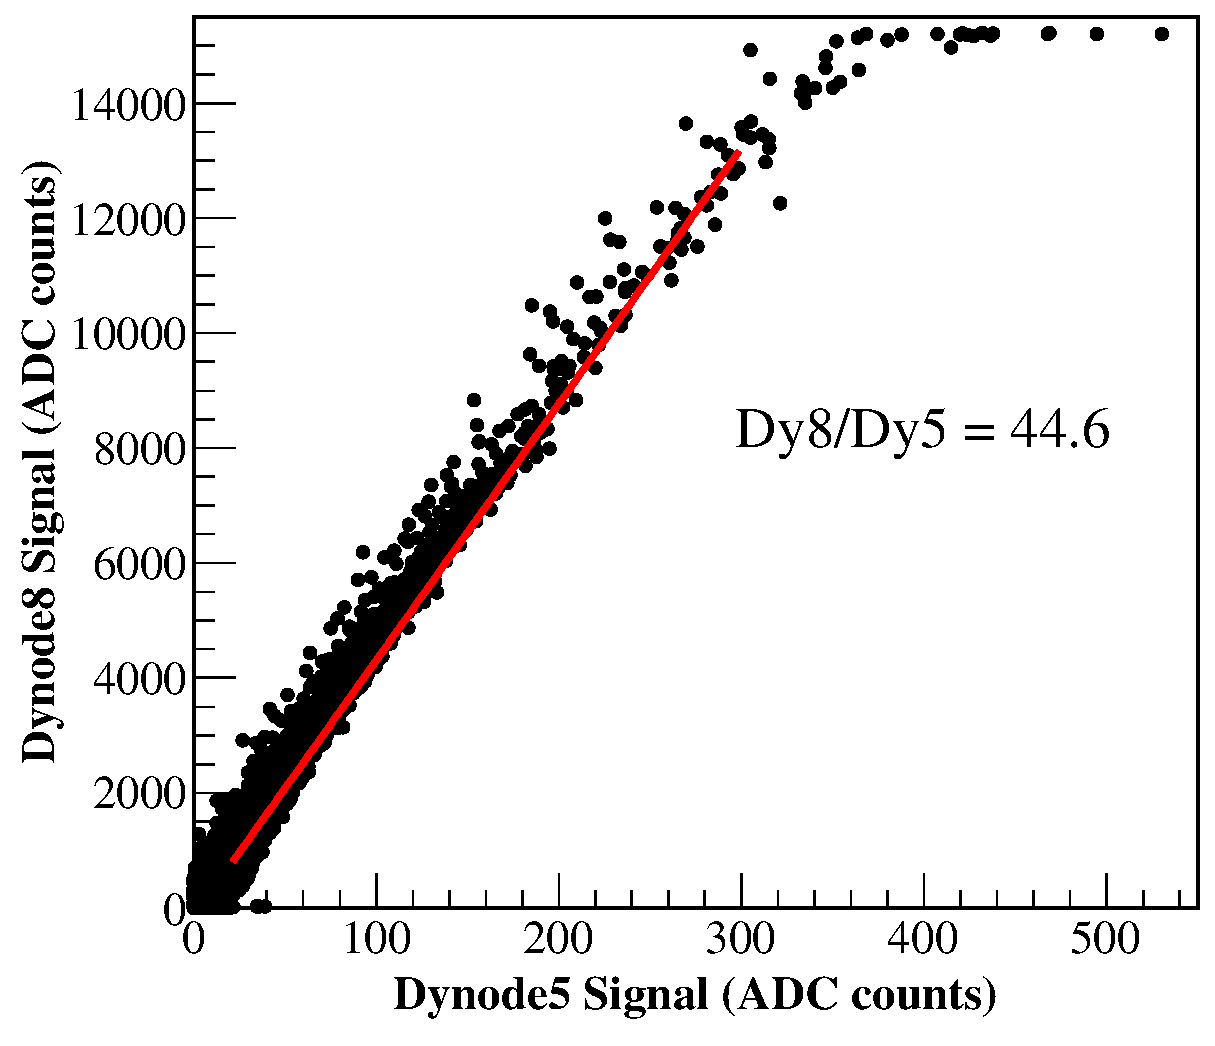
\includegraphics[width=90mm]{dy58}
\caption{The correlation between the signals in a low gain channel Dy8 and a high gain Dy5.}
\label{fig:dy58}
\end{figure} 

\subsection{Test with relativistic heavy ion beam}
\label{sec:beam}

A scintillator strip of PSD were tested at CERN SPS ion beam facility to verify our design to the required upper dynamic range. 
A primary of $^{40}Ar$($Z=18$) was accelerated to \SI{40}{AGeV\per c}, and the charge of Argon crossing the scintillator strip was measured by looking at its energy loss. 
The most probable value and the sigma of energy deposition from a relativistic Argon beam are about 217 MIPs and 4.2\% in the Fig.~\ref{fig:Ar}, respectively. 
A linear extrapolation is used to obtain the energy deposition for the Calcium ($Z=20$), and the most probable energy deposition for PSD scintillator strip is 268 MIPs from a calculation. 
Since the quenching effect existing, the actual energy deposition is a little smaller than 268 MIPs, and this value is not out of our former estimation. 
Assumption the sigma of energy deposition is 5\%, the upper limit of the amplitude of the charge pulse is 1340 MIPs as the incident Calcium particles cross the scintillator strip with the largest field view of DAMPE and a $5\sigma$ energy fluctuation is considered for the nearer readout PMT. 
This value is within the limits of our design.

\begin{figure}
 \centering
 \includegraphics[width=90mm]{Ar}
\caption{The energy deposition distribution from a relativistic $^{40}Ar$ beam.}
\label{fig:Ar}
\end{figure} 

\section{Conclusion}
\label{sec:conclustion}

A broad energy dynamic range of 0.1 MIPs$\sim$1400 MIPs required for each PSD has been deduced from a number of contributions, including energy deposition of nuclei up to charge $Z=20$, light attenuation, particle incidence angle and fluctuation of energy loss. 
A readout system that used a PMT with double dynodes output coupled to FEE with a chip VA160 optimized for positive polarity signals has been developed and used to measure the energy deposition in a scintillator strip. 
Cosmic ray muons were used to investigate the influence of scintillation light attenuation, MIPs peak and the equivalent noise of the whole detector system. 
The input noise of the whole PSD system is approximately \SI{3}{\femto\coulomb}, and the most probable value of the signal-to-noise is greater than 10 for the lower signals with 0.1 MIPs energy deposition. 
It’s also found that the required upper dynamic range 1400 MIPs could be covered by our design easily. 
A relativistic argon beam test has been also used to verify the design. 
Once again the result shows that the readout system could satisfy the large dynamic range requirements.

\subsection{summary}

\subsection{production suggestions}

%%%%%%%%%%%%%%%% Acknowledgement %%%%%%%%%%%%%%%%%%%%%%%
\section*{Acknowledgement}
\label{sec:acknowledgement}

This work was supported by the Strategic Priority Research Program on Space Science of the Chinese Academy of Science,
Grant No. XDA04040202- 3. The authors wish to thank all the people from DAMPE collaboration who helped make this work
possible.

%%%%%%%%%%%%%%%%   Bibliography  %%%%%%%%%%%%%%%%%%%%%%%
%% bibliography style
\section*{References}
\label{sec:reference}
\bibliographystyle{elsarticle-num}

%% From BibTex file
\bibliography{mybib}

\end{document}
\endinput







References

[1] T. G. Guzik, \emph{et al.}, the 26th International Cosmic Ray Conference, August, 1999.

[2] P. Picozza, \emph{et al.}, Nuclear Instruments and Methods in Physics Research A 623 (2010) 672. 

[3] M.Aguilar, \emph{et al.}, Physical Review Letters 110, (2013) 141102-1\~{}10.

[4] Chang Jin. Chin. J. Space Sci, 2014,34(5):550-557

[5] \url{http://www.eljentechnology.com/}

[6] \url{http://hamamatsu.com/}

[7] \url{http://www.dupont.com/}

[8] \href{http://pdg.lbl.gov/2014/html/authors_2014.html}{K.A.
Olive~}\href{http://pdg.lbl.gov/2014/html/authors_2014.html}{\textit{et
al.}}\href{http://pdg.lbl.gov/2014/html/authors_2014.html}{~(Particle Data Group)}, Chin. Phys. C,~38, 090001 (2014)

[9] J. B. Birks. Proc. Phys. Soc. A 64, 874 (1951).

[10] J. B. Birks. The Theory and Practice of Scintillation Counting. Pergamon Press, London, (1964).

[11] Robert DWYER, \emph{et al.}, Nuclear Instruments and Methods in Physics Research A 242 (1985) 171-176

[12] V.Bindi, \emph{et al.}, Performance of AMS-02 Time of Flight .29th International Cosmic Ray Conference Pune (2005) 9,41-44

[13] P.S.Marrocchesi, er al., Nuclear Instruments and Methods in Physics Research A 659 (2011) 477-483

[14] Katayose Y \emph{et al.} Development of High Dynamic Range Read-out System Using Multi-photodiode for the Total absorption
Calorimeter of CALET. In: 30TH International Cosmic Ray Conference. Mexico: 2008, 2(OG part 1). 437–

440

[15] Kampert K H \emph{et al.} Nuclear Instruments and Methods in Physics Research A 349 (1994) 81–95

[16] Zhang Yunlong \emph{et al.} Chinese Physics C, 2012, 36(1): 71-73

[17] Integrated Detector Electronics AS (IDEAS), VA160 datasheet, ( \url{http://www.ideas.no}).


